% !TEX TS-program = pdflatex
% !TEX root = ../ArsClassica.tex
%************************************************
%\chapter{Image Preprocessing}\label{ch:preprocessing} % 
\chapter{General Methodology}\label{ch:preprocessing} % $\mathbb{ZNR}$
%************************************************
Throughout this thesis, we will propose many analysis techniques and \ac{CAD} systems. We will apply them to many experiments, and use similar data and techniques in them. In this chapter, we will focus on the methodology that is common to most of these experiments, particularly focusing on preprocessing and evaluation of our systems. 

To perform most automated analyses on neuroimaging, it is fundamental that images are comparable. Preprocessing comprises a series of algorithms that, applied after the acquisition and reconstruction of the images, produce directly comparable images in both structure and magnitude. Whether they have been used in one or all experiments, they can be classified in two major categories: spatial and intensity preprocessing. These are addressed in Section~\ref{sec:spatial} and \ref{sec:intensityPrep} respectively. 

Afterwards, in Section~\ref{sec:validation}, we will discuss how we evaluate our systems. Here we propose some performance measures and the procedure to obtain them by training and testing our systems.  


\section{Spatial Preprocessing}\label{sec:spatial}
Spatial processing usually accounts for the differences in position, angles and structure that are commonly found between images. A common pipeline in, for example, \ac{MRI} preprocessing, is the one found at Figure~\ref{fig:examplePreMRI}, where the images are registered (or spatially normalized) to a template, smoothed and finally segmented. The smoothing is an optional step, generally used in procedures like segmentation or \ac{VBM}. 

\begin{figure}[htp]
	\myfloatalign
	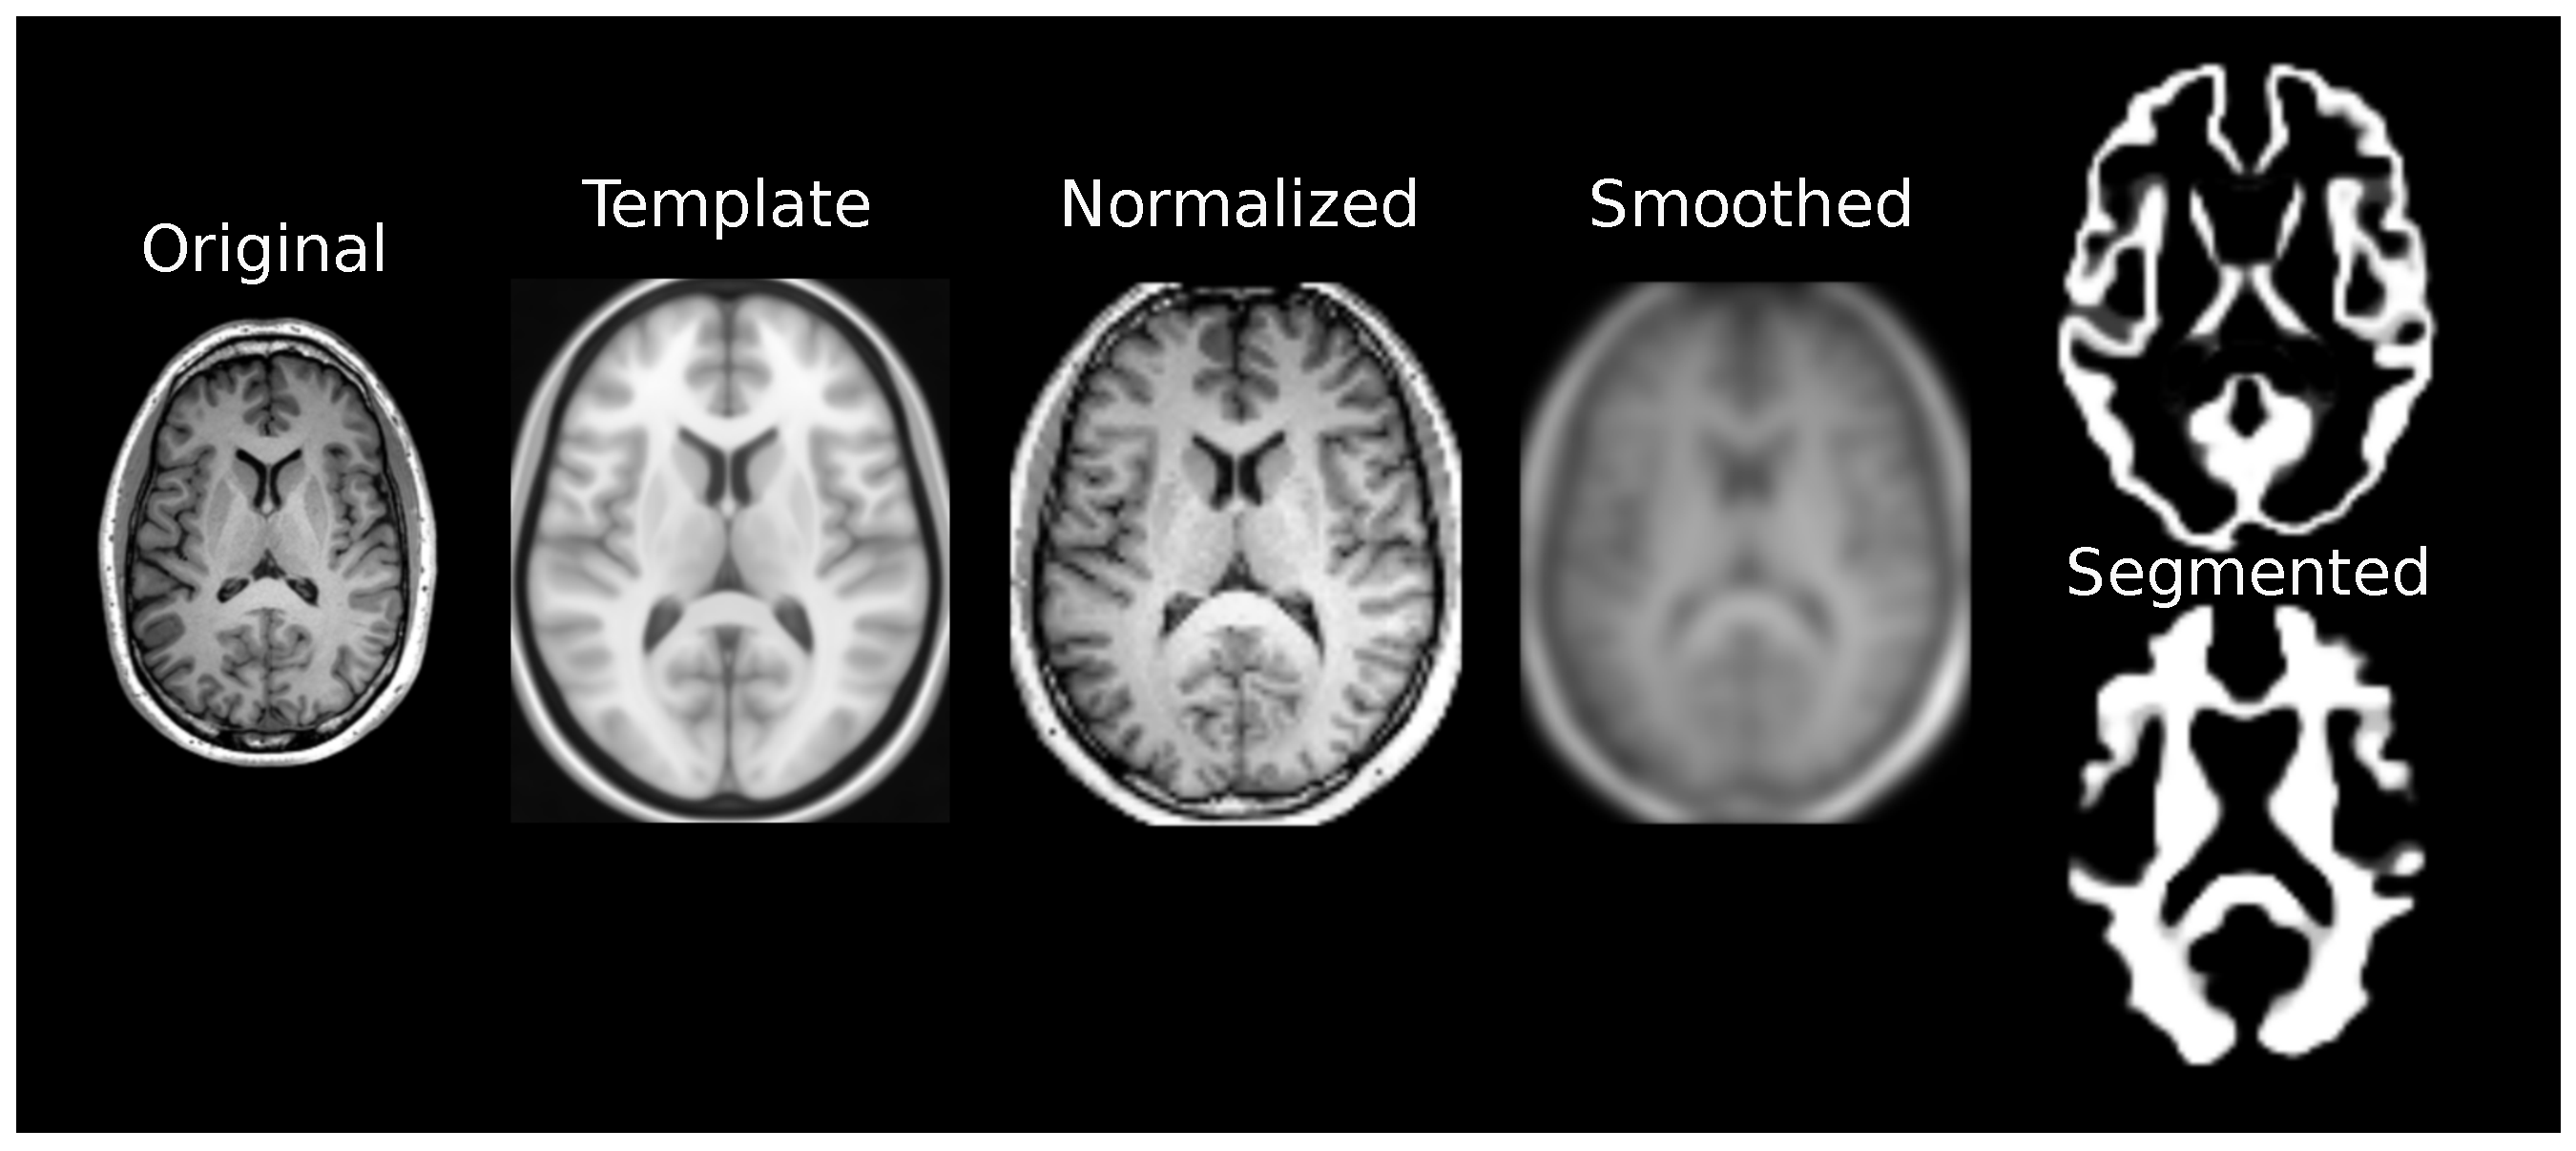
\includegraphics[width=.7\linewidth]{Graphics/ch3/preProcessPL}
	\caption[Typical pre-processing pipeline in \acs{MRI}]{Typical pre-processing pipeline in \ac{MRI}.}\label{fig:examplePreMRI}
\end{figure}

In this thesis, all the experiments in all image modalities involve spatial normalization. Smoothing, as well as segmentation, is only applied in some experiments that use \ac{MRI} images, such as the segmented images in Chapter~\ref{ch:sbm} or the whole-brain analysis performed in Chapter~\ref{ch:swpca}. 

\subsection{Spatial Normalization or Registration}
Spatial Normalization, also known as Registration, is the procedure that by which every subject's brain is mapped from their individual space to a standard reference system. Registered images allows our system to overcome the individual differences in position and anatomy by establishing a common reference space in which a given coordinate represent the same anatomical position in all brains in the dataset. 

There exist a number of pieces of software widely used for registering images, such as FreeSurfer \cite{Reuter2010} or FSL (in the FLIRT and FNIRT package) \cite{Smith2004}, most of them perform linear, non-rigid and elastic transformations or a combination of these. In this work we have used the software SPM8 \cite{spm_book} to perform registration of all the datasets, including \ac{MRI}, \ac{SPECT} and \ac{PET} images. So, from this moment, we will focus on the registration as performed in the \ac{SPM8}. 

Linear registration usually refers to the affine transformation, a matrix multiplication that includes 12 parameters for translation, rotation, scale, squeeze, shear and others: 
\begin{equation}\label{eq:affine}
	\left[\begin{matrix}
	x'\\y'\\z'\\1
	\end{matrix}\right]
	 = \left[\begin{matrix}
	 a_{00} & a_{01} & a_{02} & a_{03}\\
	 a_{10} & a_{11} & a_{12} & a_{13}\\
	 a_{20} & a_{21} & a_{22} & a_{23}\\
	 0 & 0 & 0 & 1\\
	 \end{matrix}\right]
	 \left[\begin{matrix}
	 x\\y\\z\\1
	 \end{matrix}\right]
\end{equation}

This matrix multiplication is performed globally, as it transforms the whole image, not accounting for local geometric differences. In equations \ref{eq:affine1}, \ref{eq:affine2} and \ref{eq:affine3} we give an example of the parameters that are computed for scale, translation and shear in 3D:

\begin{align}
\label{eq:affine1}
	\text{scale} &= 
	\left[\begin{matrix}
		 s_x  &0 & 0 & 0\\
		0 &s_y &0 &0\\
		0 &0 &s_z &0\\
		0 &0 &0 &1		
	\end{matrix}
	\right]\\
	\label{eq:affine2}
	\text{translation} &= 
	\left[
	\begin{matrix}
	1  &0 & 0 & \Delta x\\
	0 &1 &0 &\Delta y\\
	0 &0 &1 &\Delta z\\
	0 &0 &0 &1		
	\end{matrix}
	\right] \\
	\label{eq:affine3}
	\text{shear} &= 
	\left[\begin{matrix}
	1  &h_{xy}& h_{xz} & 0\\
	h_{yx} &1 &h_{yz} &0\\
	h_{zx} &h_{zy} &1 &0\\
	0 &0 &0 &1		
	\end{matrix}
	\right]
\end{align}

The combination of all these operations result in the estimation of the twelve parameters that we found in Eq.~\ref{eq:affine}, which are the ones used in \ac{SPM8}. The estimation of these parameters is performed via the optimization of a cost function, that in \ac{SPM8} can be the minimum squared difference between the source image and the template \cite{spm_book} in the case of within-modality registration, or the mutual information in between-modality registration. These functions are also used in FLIRT \cite{Jenkinson2001}, whereas FreeSurfer uses the Tukey's biweight function (in {\ttfamily mri\_robust\_template}) \cite{Reuter2012}.

After the affine transform, the software usually performs a fine-tuning step via nonrigid transformations, to account for relevant a\-na\-to\-mi\-cal differences between subjects. Nonrigid transformations range from the use of radial basis functions, physical continuum models and the large deformation models, or diffeomorphisms, that \ac{SPM8} uses. These procedures work by estimating a warp-field and then, apply it to the affine-registered images. An example of the differences of using only affine registration and applying diffeomorphisms can be found at Figure~\ref{fig:diffeomorphisms}.

\begin{figure}[bth]
	\myfloatalign
	\subfloat[Comparison in \ac{MRI}.]
	{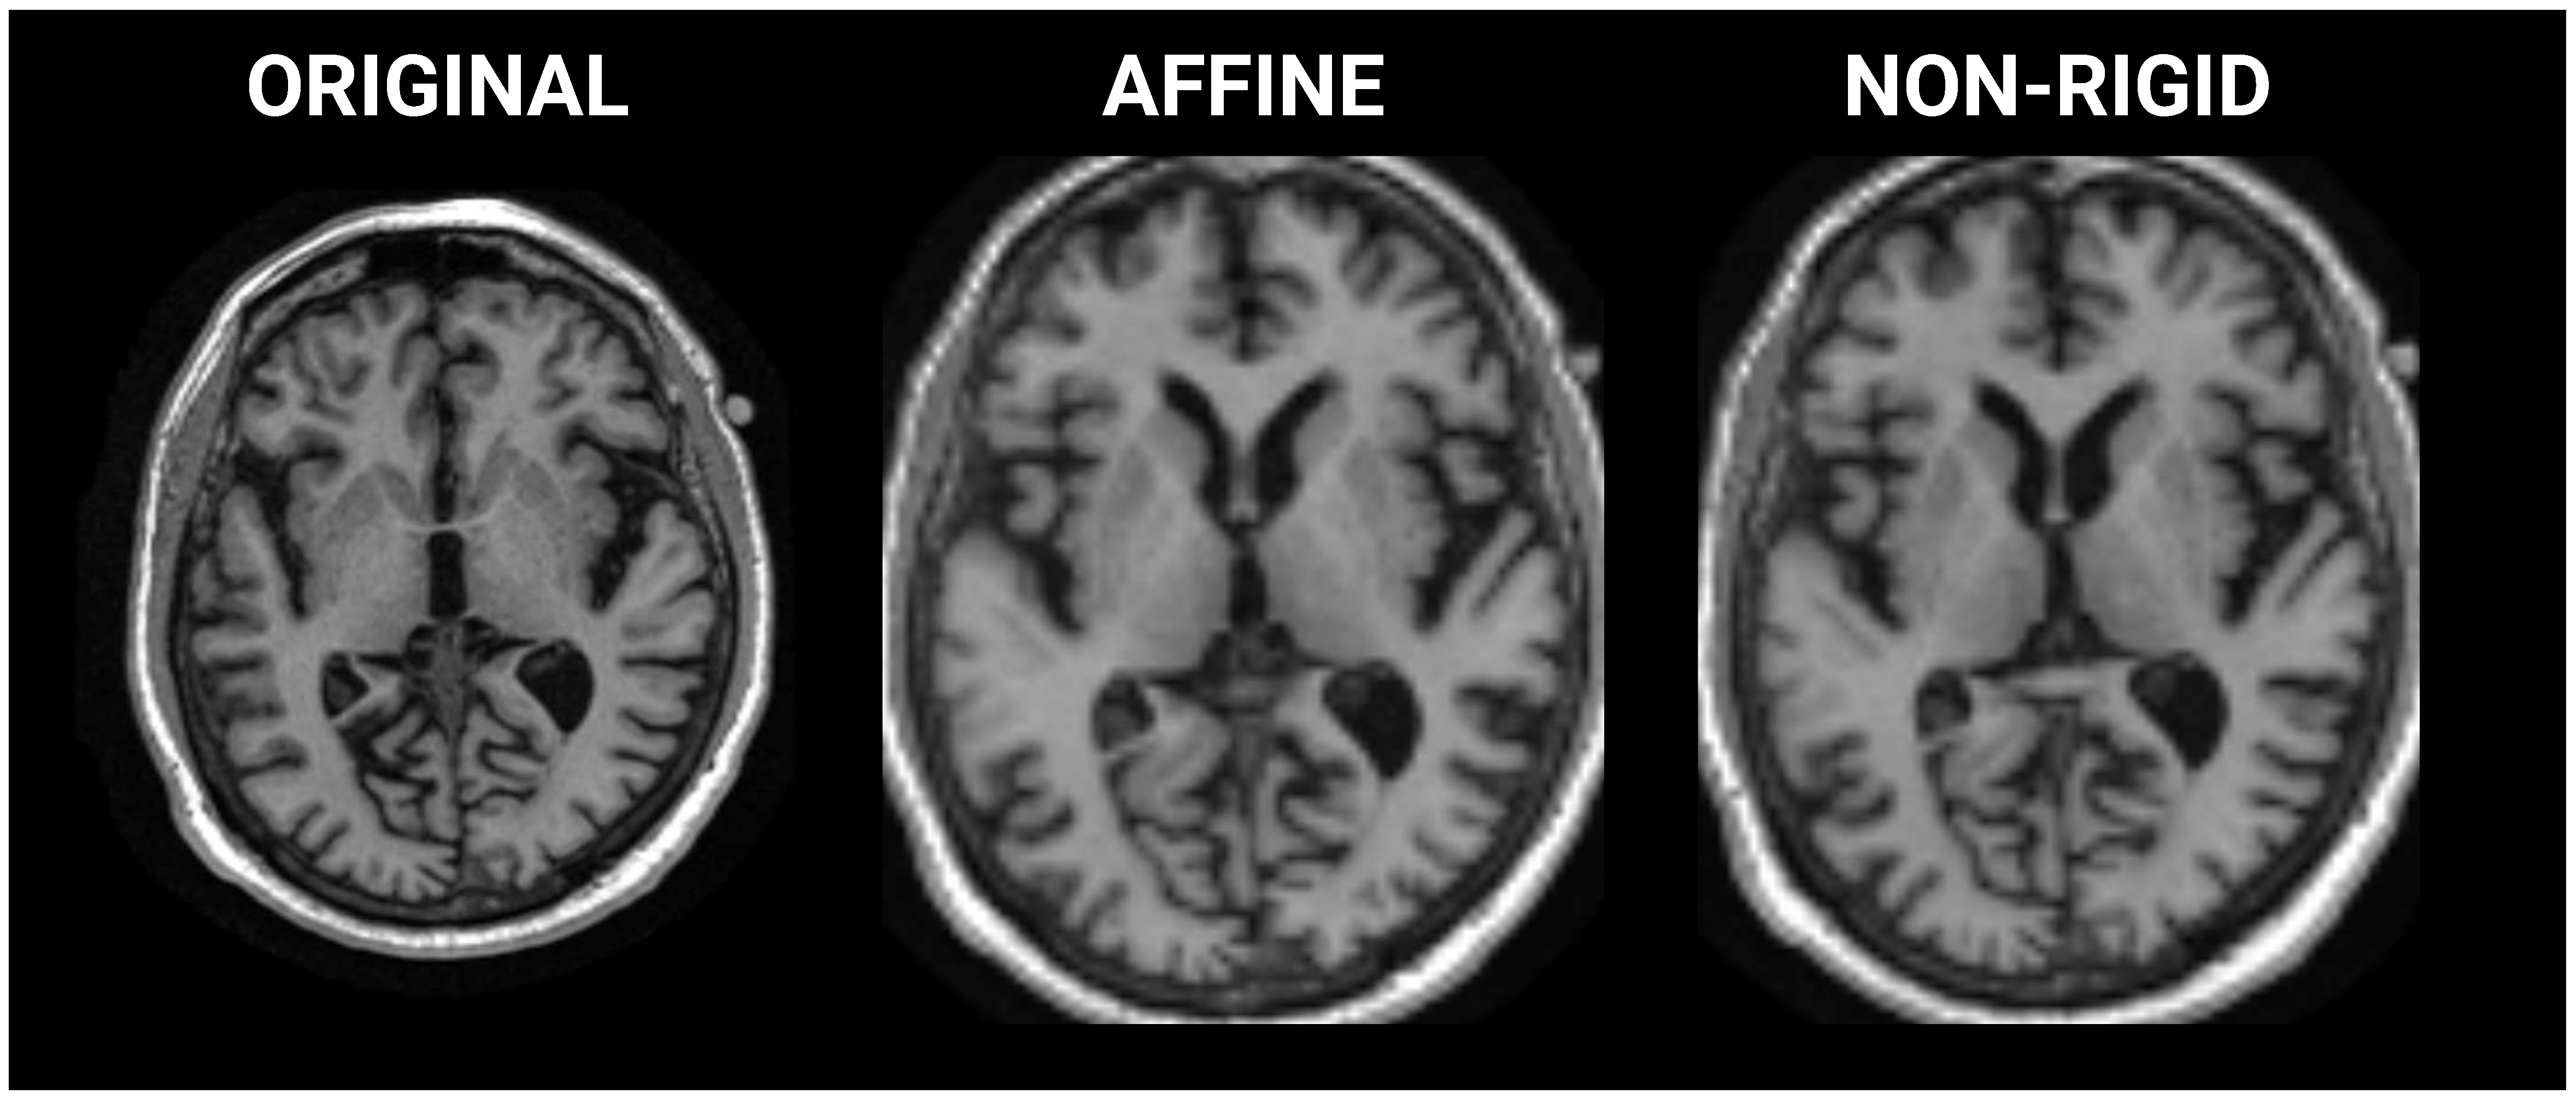
\includegraphics[width=.7\linewidth]{Graphics/ch3/regComparisonMRI}}
	 \\
	\subfloat[Comparison in \ac{PET}.]
	{\includegraphics[width=.7\linewidth]{Graphics/ch3/regComparisonPET}}
	\caption[Comparison of the affine registration and the application of non-linear transformations to the images]{Comparison of the affine registration and the application of non-linear transformations to both \ac{MRI} and \ac{PET} images of the same \ac{ADNI} subject.}\label{fig:diffeomorphisms}
\end{figure}


\subsubsection{Co-registration}
Sometimes we have several image modalities of the same subject, for example \ac{MRI} and \ac{PET} or functional \ac{MRI}, often acquired at the same time. In this particular case, we can use the higher resolution \ac{MRI} image to calculate the affine parameters and warping, and apply those to all modalities of the same subject. To do so, we perform a first co-registration, that is, a registration of the lower-resolution images (e.g. \ac{PET}) to its correspondent \ac{MRI} image. Being anatomically similar, the co-registration usually comprises a single affine transformation. Afterwards, we can proceed with the registration of that \ac{MRI} image to the template, and apply the same transformation to all its co-registered images. 

\subsubsection{The MNI Space}
In this thesis, all images are coregistered to the \acf{MNI} space \cite{Mazziotta2001}. This is the most widely used coordinate system, recently adopted by the International Consortium for Brain Mapping (ICBM) as its standard template. The three-dimensional coordinate system defined in \ac{MNI} was intended to replace the Tailarach space, a system based on a dissected brain, that was used to compose an atlas by Tailarach and Tournoux \cite{Talairach1988c}. The current template is known as ICBM152, and features the average of 152 normal \ac{MRI} scans matched to an older \ac{MNI} template using a nine parameter affine registration. 

\subsection{Segmentation}
When using \ac{MRI} images in this thesis, we often refer to \acf{GM} and \acf{WM} maps, which is the result of the segmentation of the original data. Segmentation aims at producing maps of the distribution of different tissues, and it generally addresses \ac{GM}, \ac{WM} and \ac{CSF} classes, although lately some software can output data for bone, soft tissue or very detailed functional regions and subregions \cite{Fischl2002}. 

In this thesis we have used the \ac{VBM} toolbox of the \ac{SPM8} software, which yields \ac{GM}, \ac{WM} and \ac{CSF} maps. It features an \ac{EM} algorithm to model the distribution of the tissue classes as a mixture of gaussians and, by combining this distribution-based information with tissue probability maps using a bayesian rule, the software produces joint posterior probability maps for each tissue. To clean up the segmentation maps, a series of iterative dilations and erosions are used. Finally, since brain regions are expanded or contracted at the spatial normalization step, we can scale the segmented maps using modulation, producing final maps where the total amount of grey matter is preserved. 

\section{Intensity Normalization}\label{sec:intensityPrep}
Generally, structural modalities such as T1 and T2-weighted images are considered unitless, in contrast to functional imaging, in which each voxel's intensity represent the distribution of some biomarker, such as glucose metabolism, dopamine transporters, etc. These amounts are affected by many sources of variability that can affect the final values: contrast uptake, radiotracer decay time, metabolism, etc. Therefore, along with the previous spatial normalization, there is a need to normalize the intensities of the images, so that the amount they represent are comparable. 

In the case of intensity normalization, the method acts as a linear transformation of the image, preserving fundamental information such as contrast between regions. This approximation estimates the new intensity values $I'$ as: 
\begin{equation}
	I' = I/I_p 
\end{equation}
where $I_p$ is a constant parameter that is unique for each image. After this division, the new intensities would be directly comparable. The technique used to compute the normalization parameter varies, ranging from the simplest normalization to the maximum \cite{Salas-Gonzalez2009,Martinez-Murcia20129676} to complex methodologies that use assumptions about the image's \ac{PDF}. 

The \emph{normalization to the maximum} strategy computes $I_p$ as the average value of the 95th bin of the histogram of the image. In other words, this mean averaging the 5\% higher intensity values and use this mean as $I_p$. Another useful approach is the so-called \emph{integral normalization}, which computes $I_p$ as the sum of all values in the image. 

Other approaches involves some a-priori knowledge about the intensity distribution of normal subjects in a certain modality. This is the case of setting $I_p$ to the Binding Potential (BP), a ratio between the intensities at specific and non-specific areas \cite{Scherfler2005}. 

Finally, more advanced approaches use a general linear transformation of the image: 
\begin{equation}
	I' = a I + b
\end{equation}
The parameters $a$ and $b$ are so that the \ac{PDF} of a given matches a reference \ac{PDF}. There exist methods that use the histogram \cite{Arndt1996}, the gaussian distribution or the alpha-stable distribution \cite{Salas-Gonzalez2013}. In this latter case, the parameters $a$ y $b$ are computed as linear transformations of some distribution's parameters: 
\begin{equation}
	a = \frac{\gamma*}{\gamma}, \quad b = \mu* + \frac{\gamma*}{\gamma} \mu
\end{equation}
where $\gamma*$ and $\gamma$ are the dispersion parameters of the alpha-stable intensity distribution of the non-normalized and the reference image respectively, and $\mu*$ and $\mu$ are the location parameters of the same images. 

Despite traditionally structural modalities such as \ac{MRI} did not use intensity normalization, there exist a new tendency towards the use of \ac{qT1} and \ac{qT2} images \cite{Weiskopf2013} that provide biomarkers for absolute measures such as myelination, water and iron levels. This strategy is especially designed to overcome different sources of variability that affect multicentre studies, e.g. magnetic field inhomogeneity, noise, evolution of the scanners, etc. The role of those in multi-centre studies is addressed at Chapter~\ref{ch:swpca}. 

See Figure~\ref{fig:comparisonIntNorm} for a comparison between different strategies of intensity normalization on the same images. 

\begin{figure}[bth]
	\myfloatalign
	\subfloat[No Normalization.]
	{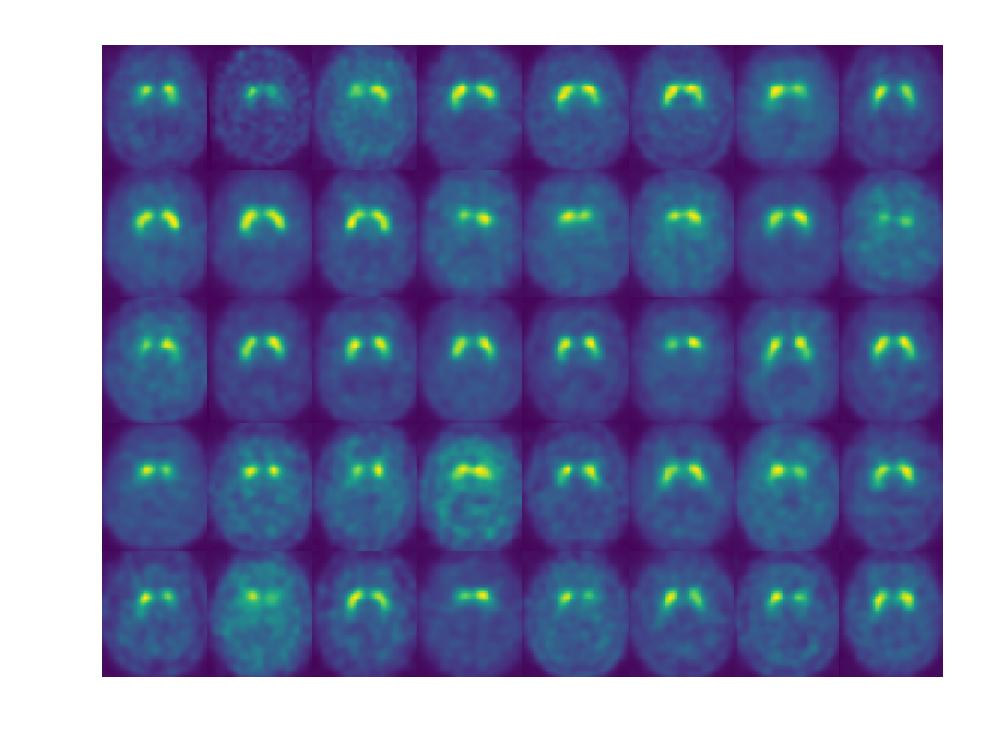
\includegraphics[width=.45\linewidth]{Graphics/ch3/norm_no.eps}}
	\subfloat[Normalization to the Maximum.]
	{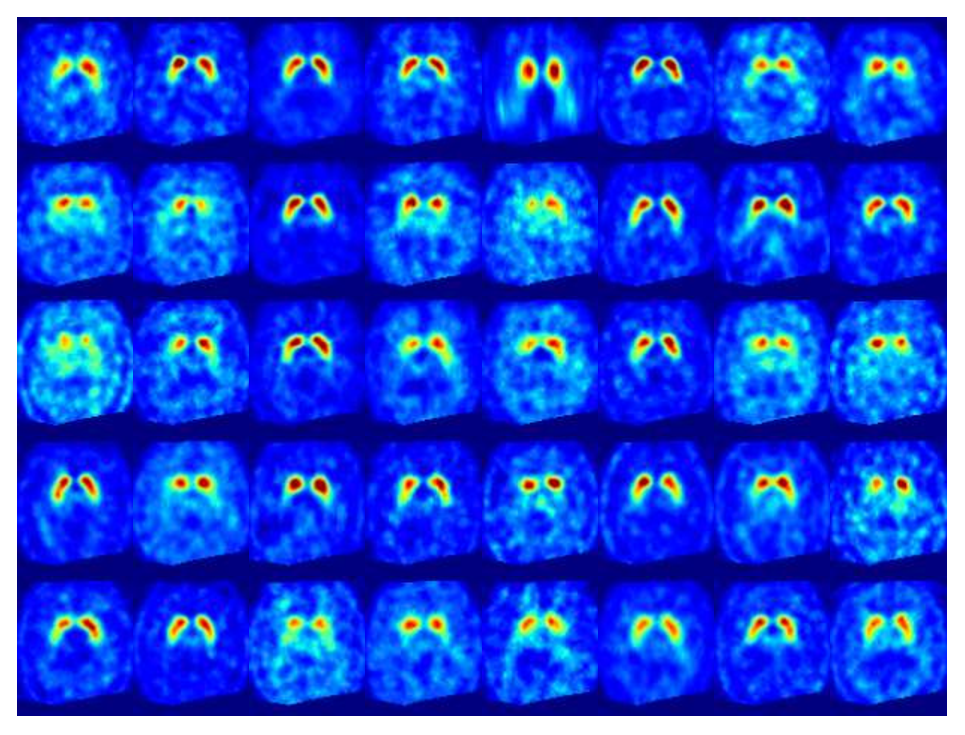
\includegraphics[width=.45\linewidth]{Graphics/ch3/norm_max.eps}}\\
	\subfloat[Integral Normalization.]
	{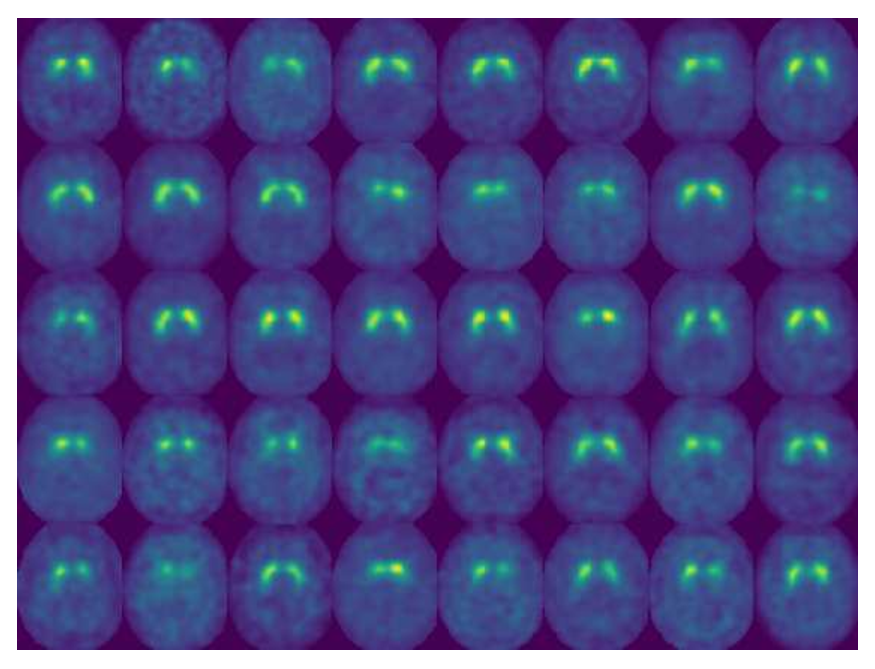
\includegraphics[width=.45\linewidth]{Graphics/ch3/norm_int.eps}}
	\subfloat[Normalization using $\alpha$-stable distribution.]
	{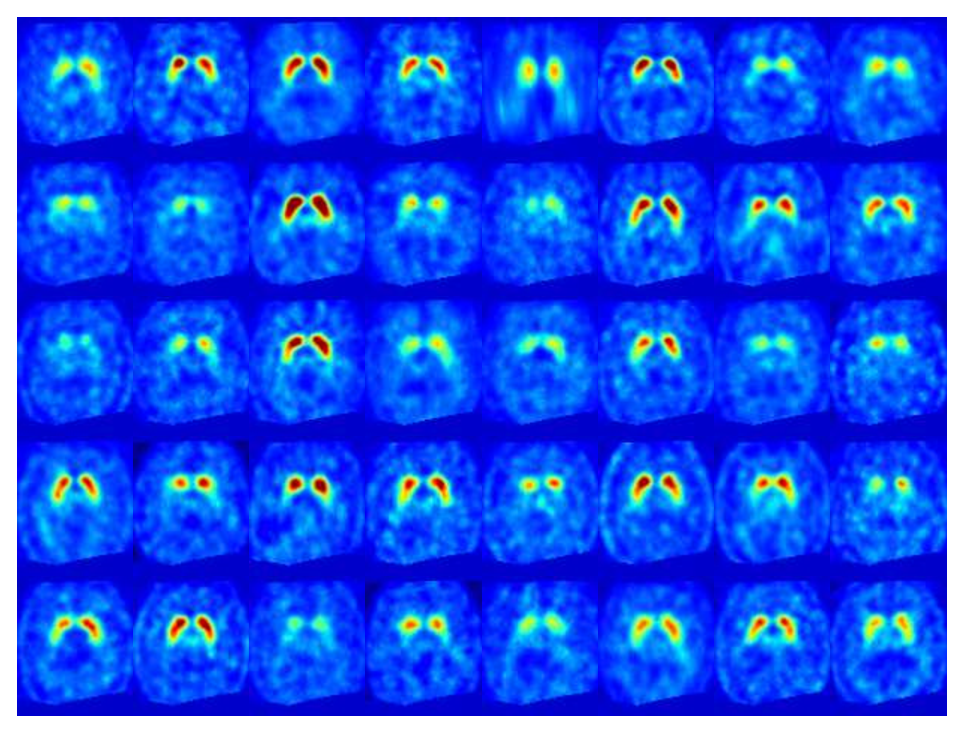
\includegraphics[width=.45\linewidth]{Graphics/ch3/norm_est.eps}}
	\caption[Comparison between different types of intensity normalization.]{Comparison between different types of intensity normalization, applied to the VDLN-DAT dataset (see Appendix~\ref{ch:datasets}).}\label{fig:comparisonIntNorm}
\end{figure}
%DONE

\section{Evaluation Parameters and Methodology}\label{sec:validation}
\subsection{Cross-validation}
Some machine learning applications such as digit or faces recognition use tens of thousands of images as input. In these cases, the common practice is to divide randomly the data in three subsets: training, validation and testing \cite{Bradley1997}. However, in neuroimaging, sample size is an issue. In contrast to those applications, we only have hundreds of patients in the best case, and the estimation of the performance using these subsets might not be reliable. 
 
In these cases, \acf{CV} is used to obtain more accurate performance measures. \ac{CV} performs a division of the dataset into several subsets $X = {S_1, S_2, ... S_k}$ and iteratively use some of these subsets for training or testing. The simplest \ac{CV} estimator is $k$-fold. This approach uses $k$ equally-sized, non-overlapping subset. For each subset $S_i$ (or ``fold'', hence the name), the model is trained on all subsets $S_k \forall k \neq i$, and then evaluated on $S_i$. The performance measures, \eg accuracy, are obtained as the average of the accuracies on each fold. 

A particular case where $k=N$ (where $N$ is the exact number of subjects in the dataset) is \acf{LOO}. This estimator is approximately unbiased for the true accuracy, but can have high variance because there is much overlapping between the $N$ training set \cite{Hastie2009}. This imply that the learned models are correlated, and therefore, dependent. All \ac{CV} strategies with $k>2$ have overlap, and therefore, high variance. See how variance and bias evolve in a $k$-fold validation in Figure~\ref{fig:evolutionKFold}. 

\begin{figure}
\centering
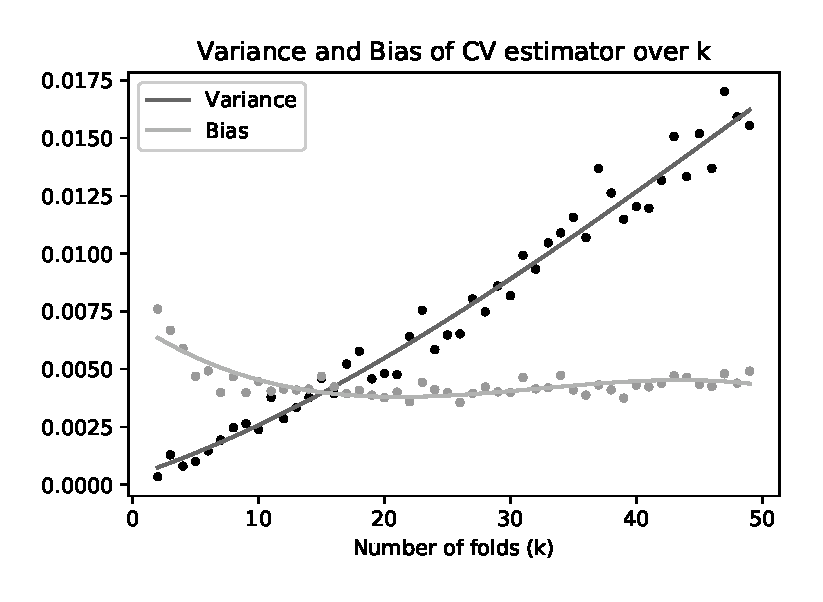
\includegraphics[width=0.7\linewidth]{Graphics/ch3/evolutionKFold}
\caption[Evolution of bias and variance in \acs{CV}.]{Evolution of bias and variance when increasing the number of folds in a $k$-fold \ac{CV}.}
\label{fig:evolutionKFold}
\end{figure}


Using $k=10$ is assumed as a good compromise between variance and bias in many works \cite{Kohavi1995,Hastie2009}. In this thesis, when referring to $k$-fold, we often use stratified cross validation, which is a subclass of $k$-fold where the distribution of classes within each fold is similar to the distribution of classes in the whole dataset, making the estimates more accurate \cite{Kohavi1995}. 
\subsection{Classification Performance}
From each iteration in the \ac{CV} loop, a confusion matrix is obtained, from which all performance measures will be obtained. 

\begin{table}
	\myfloatalign
	\begin{tabular}{cc|c|c|}
		\cline{3-4}
		& & \multicolumn{2}{c|}{Predicted}\\
		\cline{3-4}
		& &  Positive & Negative \\ 
		\hline
		\multicolumn{1}{ |c  }{\multirow{2}{*}{Actual}}& \multicolumn{1}{ |c|  }{Positive} & True Positive & False Positive \\ 
		\cline{2-4}
		\multicolumn{1}{ |c  }{} &  \multicolumn{1}{ |c|  }{Negative} & False Negative & True Negative  \\ 
		\hline
	\end{tabular} 
	\caption{Confusion matrix and its parts}
	\label{tab:confmat}
\end{table}

The confusion matrix (see Table~\ref{tab:confmat}) accounts for the number of correct and incorrect predictions: \acp{TP} and \acp{TN} are correct predictions, and \acp{FP} and \acp{FN} are incorrect predictions. It also allow us to identify which type of error is our model making, which in hypothesis testing are known as type I errors( \acp{FP}) and type II errors (\acp{FN}). The confusion matrix is the basis for computing other performance measures, such as accuracy (acc), sensitivity (sens) or specificity (spec).

\begin{align}
\text{acc} & = \frac{TP + TN}{TP + TN + FP + FN}\\
\text{sens} & = \frac{TP}{TP + FN}\\
\text{spec} & = \frac{TN}{TN + FP}
\end{align}

Sensitivity is also known as \ac{TP} rate or recall in the literature, and specificity is known as \ac{TN} rate. Sensitivity is widely used in the medical literature, since it gives an idea of how ``sensitive'' is our model to the patterns related to a disease (usually considered the positive). 
